% chktex-file 8

\documentclass{article}
\usepackage{amsmath}
\usepackage[a4paper, top=0.75in, bottom=0.75in]{geometry}
\usepackage{enumitem}
\usepackage{tikz}
\usepackage{graphicx}

\graphicspath{ {./images/} }

\title{Midterm Exam 1}
\author{David Robinson}
\date{}
\setlength{\parindent}{0pt}

\begin{document}

\maketitle

\subsection*{Problem 1}

\[{(a\cup d)}^* c{(b{(dd)}^*\cup c\cup d)}^* b\]

\subsection*{Problem 2}

Let $M$ be a DFA that recognizes $L$. We can construct an NFA $M'$ to recognize $h(L)$ by replacing each transition $\delta(q,a)$ in $M$ with a sequence of transitions in $M'$ that process $h(a)$ instead of $a$. Since NFAs and DFAs both define the class of regular languages, the resulting language $h(L)$ is regular. Therefore, regular languages are closed under homomorphism.


\subsection*{Problem 3}

\begin{center}
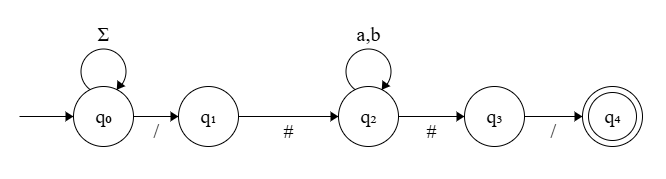
\includegraphics[scale=0.5]{exam1-1.png}
\end{center}

\subsection*{Problem 4}

If $L=\{ccc\#cc\#c\text{ with } c\in{\{a,b\}}^*\}$ is a regular language, then it must satisfy the Pumping Lemma, where there exists a pumping length $p$ such that any string $s$ in $L$ with $|s|\geq p$ can be split into $s=xyz$ where:
\begin{enumerate}
    \item $xy^k z\in L$ for all $k\geq 0$
    \item $|y|>0$
    \item $|xy|\leq p$
\end{enumerate}

Consider a string $s=a^p b^p a^p b^p a^p b^p\#a^p b^p a^p b^p\#a^p b^p$ in $L$ where $c=a^p b^p$. Pumping $y$ increases the number of $a$'s only in the first $c$, while the other instances of $c$ are unchanged. Since the resulting string no longer follows the pattern $ccc\#cc\#c$, it contradicts the Pumping Lemma and $L$ is not a regular language.
\subsection*{Problem 5}

\begin{center}
    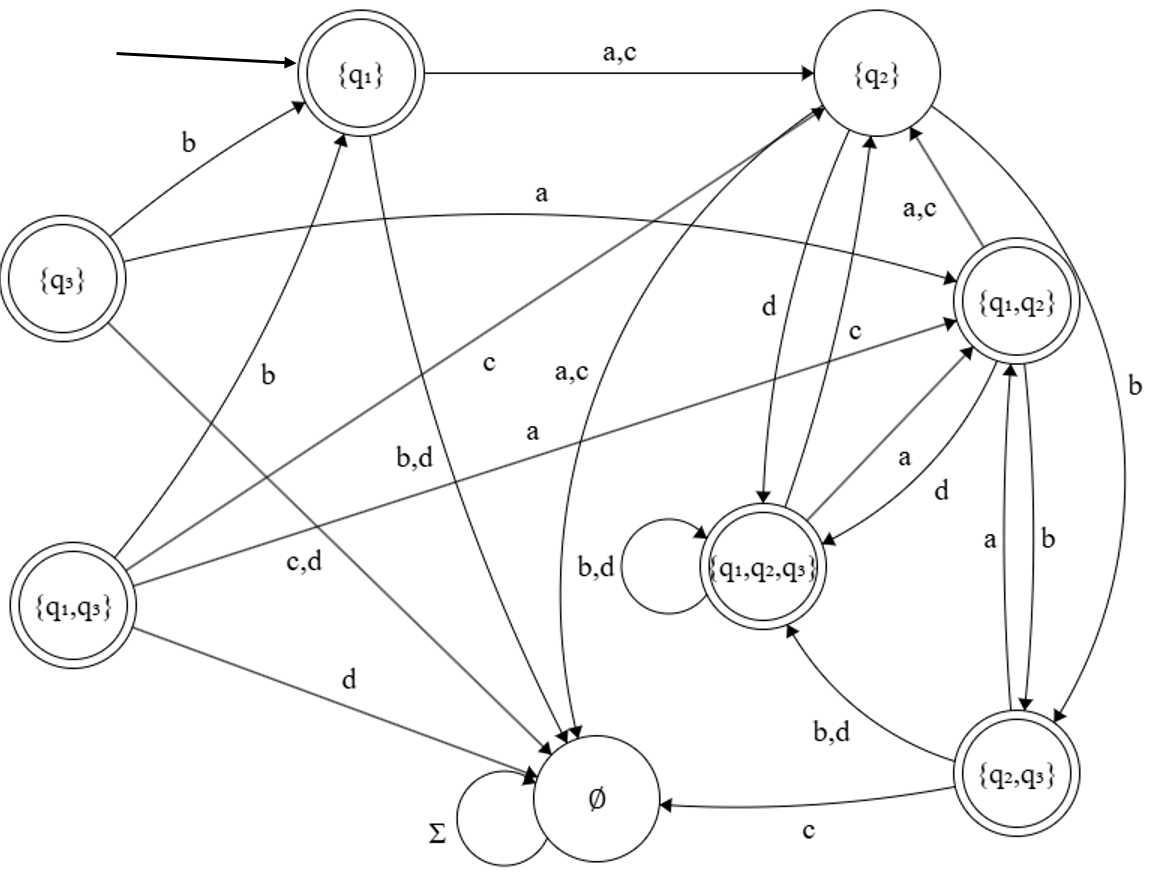
\includegraphics[scale=0.36]{exam1-2.png}
\end{center}

\subsection*{Problem 6}

\begin{center}
    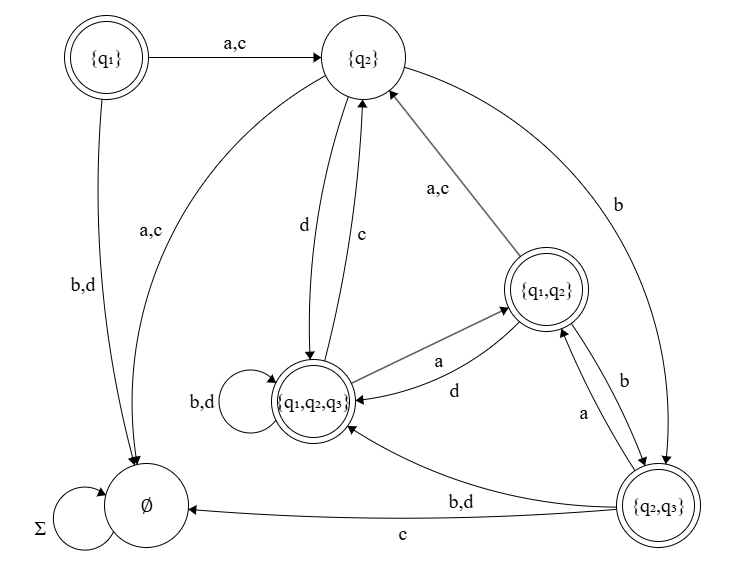
\includegraphics[scale=0.38]{exam1-3.png}
\end{center}

\subsection*{Problem 7}

% \[{\Big[(b\cup d)(b\cup d)\cup \big[[(a\cup c)\cup(b\cup d)(a\cup c)]{[(a\cup c)(a\cup c)]}^*[(b\cup d)\cup (a\cup c)(b\cup d)]\big]\Big]}^*\]
\begin{center}
    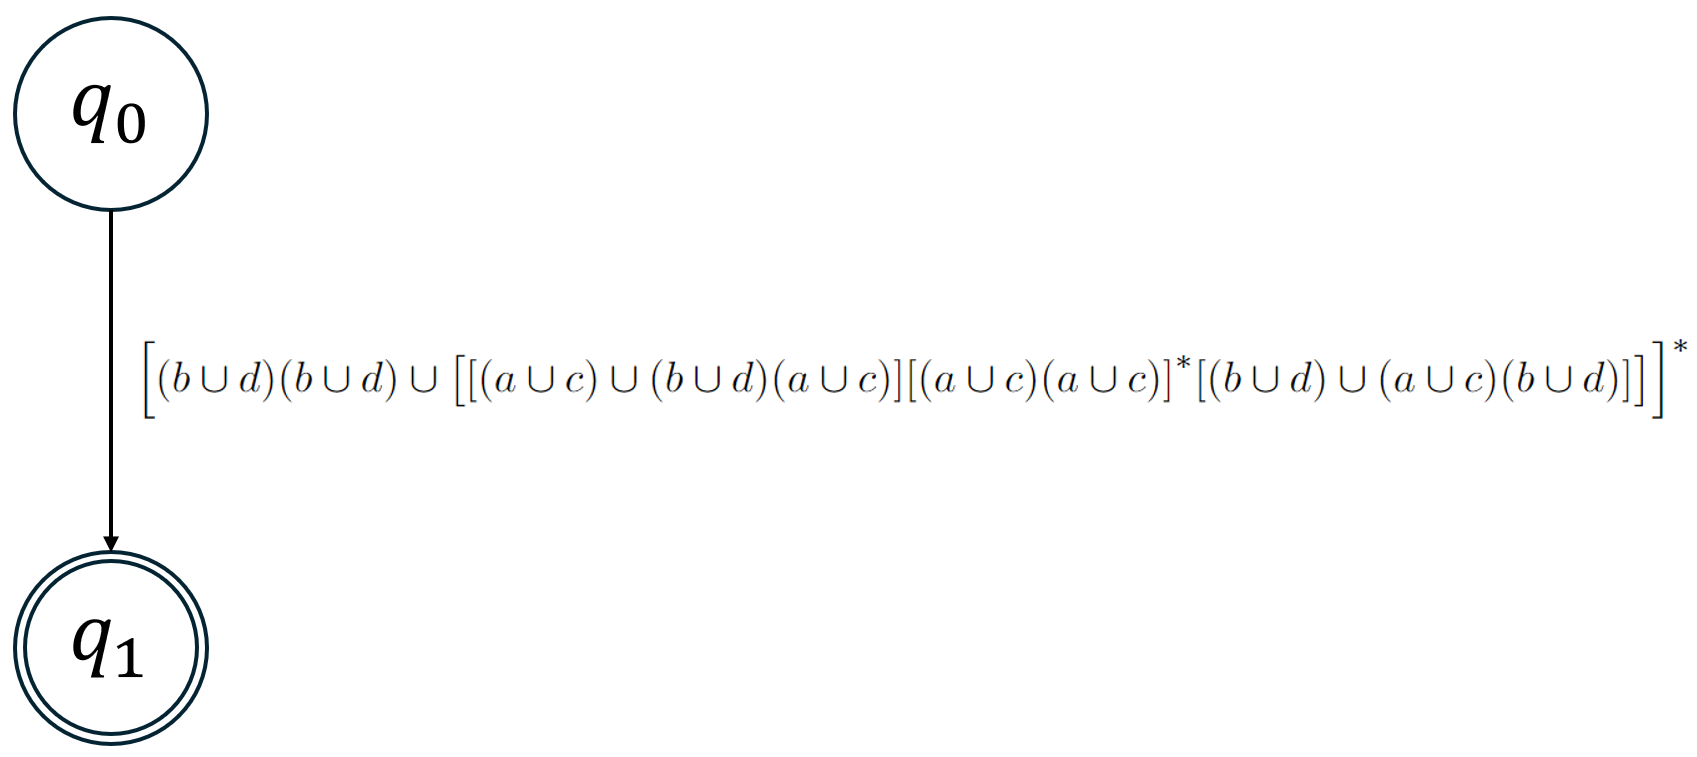
\includegraphics[scale=0.24]{exam1-4.png}
\end{center}

\end{document}